% Options for packages loaded elsewhere
\PassOptionsToPackage{unicode}{hyperref}
\PassOptionsToPackage{hyphens}{url}
%
\documentclass[
]{book}
\usepackage{amsmath,amssymb}
\usepackage{lmodern}
\usepackage{iftex}
\ifPDFTeX
  \usepackage[T1]{fontenc}
  \usepackage[utf8]{inputenc}
  \usepackage{textcomp} % provide euro and other symbols
\else % if luatex or xetex
  \usepackage{unicode-math}
  \defaultfontfeatures{Scale=MatchLowercase}
  \defaultfontfeatures[\rmfamily]{Ligatures=TeX,Scale=1}
\fi
% Use upquote if available, for straight quotes in verbatim environments
\IfFileExists{upquote.sty}{\usepackage{upquote}}{}
\IfFileExists{microtype.sty}{% use microtype if available
  \usepackage[]{microtype}
  \UseMicrotypeSet[protrusion]{basicmath} % disable protrusion for tt fonts
}{}
\makeatletter
\@ifundefined{KOMAClassName}{% if non-KOMA class
  \IfFileExists{parskip.sty}{%
    \usepackage{parskip}
  }{% else
    \setlength{\parindent}{0pt}
    \setlength{\parskip}{6pt plus 2pt minus 1pt}}
}{% if KOMA class
  \KOMAoptions{parskip=half}}
\makeatother
\usepackage{xcolor}
\IfFileExists{xurl.sty}{\usepackage{xurl}}{} % add URL line breaks if available
\IfFileExists{bookmark.sty}{\usepackage{bookmark}}{\usepackage{hyperref}}
\hypersetup{
  pdftitle={Start R},
  pdfauthor={Vincent Bonhomme},
  hidelinks,
  pdfcreator={LaTeX via pandoc}}
\urlstyle{same} % disable monospaced font for URLs
\usepackage{color}
\usepackage{fancyvrb}
\newcommand{\VerbBar}{|}
\newcommand{\VERB}{\Verb[commandchars=\\\{\}]}
\DefineVerbatimEnvironment{Highlighting}{Verbatim}{commandchars=\\\{\}}
% Add ',fontsize=\small' for more characters per line
\usepackage{framed}
\definecolor{shadecolor}{RGB}{248,248,248}
\newenvironment{Shaded}{\begin{snugshade}}{\end{snugshade}}
\newcommand{\AlertTok}[1]{\textcolor[rgb]{0.94,0.16,0.16}{#1}}
\newcommand{\AnnotationTok}[1]{\textcolor[rgb]{0.56,0.35,0.01}{\textbf{\textit{#1}}}}
\newcommand{\AttributeTok}[1]{\textcolor[rgb]{0.77,0.63,0.00}{#1}}
\newcommand{\BaseNTok}[1]{\textcolor[rgb]{0.00,0.00,0.81}{#1}}
\newcommand{\BuiltInTok}[1]{#1}
\newcommand{\CharTok}[1]{\textcolor[rgb]{0.31,0.60,0.02}{#1}}
\newcommand{\CommentTok}[1]{\textcolor[rgb]{0.56,0.35,0.01}{\textit{#1}}}
\newcommand{\CommentVarTok}[1]{\textcolor[rgb]{0.56,0.35,0.01}{\textbf{\textit{#1}}}}
\newcommand{\ConstantTok}[1]{\textcolor[rgb]{0.00,0.00,0.00}{#1}}
\newcommand{\ControlFlowTok}[1]{\textcolor[rgb]{0.13,0.29,0.53}{\textbf{#1}}}
\newcommand{\DataTypeTok}[1]{\textcolor[rgb]{0.13,0.29,0.53}{#1}}
\newcommand{\DecValTok}[1]{\textcolor[rgb]{0.00,0.00,0.81}{#1}}
\newcommand{\DocumentationTok}[1]{\textcolor[rgb]{0.56,0.35,0.01}{\textbf{\textit{#1}}}}
\newcommand{\ErrorTok}[1]{\textcolor[rgb]{0.64,0.00,0.00}{\textbf{#1}}}
\newcommand{\ExtensionTok}[1]{#1}
\newcommand{\FloatTok}[1]{\textcolor[rgb]{0.00,0.00,0.81}{#1}}
\newcommand{\FunctionTok}[1]{\textcolor[rgb]{0.00,0.00,0.00}{#1}}
\newcommand{\ImportTok}[1]{#1}
\newcommand{\InformationTok}[1]{\textcolor[rgb]{0.56,0.35,0.01}{\textbf{\textit{#1}}}}
\newcommand{\KeywordTok}[1]{\textcolor[rgb]{0.13,0.29,0.53}{\textbf{#1}}}
\newcommand{\NormalTok}[1]{#1}
\newcommand{\OperatorTok}[1]{\textcolor[rgb]{0.81,0.36,0.00}{\textbf{#1}}}
\newcommand{\OtherTok}[1]{\textcolor[rgb]{0.56,0.35,0.01}{#1}}
\newcommand{\PreprocessorTok}[1]{\textcolor[rgb]{0.56,0.35,0.01}{\textit{#1}}}
\newcommand{\RegionMarkerTok}[1]{#1}
\newcommand{\SpecialCharTok}[1]{\textcolor[rgb]{0.00,0.00,0.00}{#1}}
\newcommand{\SpecialStringTok}[1]{\textcolor[rgb]{0.31,0.60,0.02}{#1}}
\newcommand{\StringTok}[1]{\textcolor[rgb]{0.31,0.60,0.02}{#1}}
\newcommand{\VariableTok}[1]{\textcolor[rgb]{0.00,0.00,0.00}{#1}}
\newcommand{\VerbatimStringTok}[1]{\textcolor[rgb]{0.31,0.60,0.02}{#1}}
\newcommand{\WarningTok}[1]{\textcolor[rgb]{0.56,0.35,0.01}{\textbf{\textit{#1}}}}
\usepackage{longtable,booktabs,array}
\usepackage{calc} % for calculating minipage widths
% Correct order of tables after \paragraph or \subparagraph
\usepackage{etoolbox}
\makeatletter
\patchcmd\longtable{\par}{\if@noskipsec\mbox{}\fi\par}{}{}
\makeatother
% Allow footnotes in longtable head/foot
\IfFileExists{footnotehyper.sty}{\usepackage{footnotehyper}}{\usepackage{footnote}}
\makesavenoteenv{longtable}
\usepackage{graphicx}
\makeatletter
\def\maxwidth{\ifdim\Gin@nat@width>\linewidth\linewidth\else\Gin@nat@width\fi}
\def\maxheight{\ifdim\Gin@nat@height>\textheight\textheight\else\Gin@nat@height\fi}
\makeatother
% Scale images if necessary, so that they will not overflow the page
% margins by default, and it is still possible to overwrite the defaults
% using explicit options in \includegraphics[width, height, ...]{}
\setkeys{Gin}{width=\maxwidth,height=\maxheight,keepaspectratio}
% Set default figure placement to htbp
\makeatletter
\def\fps@figure{htbp}
\makeatother
\setlength{\emergencystretch}{3em} % prevent overfull lines
\providecommand{\tightlist}{%
  \setlength{\itemsep}{0pt}\setlength{\parskip}{0pt}}
\setcounter{secnumdepth}{5}
\usepackage{booktabs}
\usepackage{amsthm}
\makeatletter
\def\thm@space@setup{%
  \thm@preskip=8pt plus 2pt minus 4pt
  \thm@postskip=\thm@preskip
}
\makeatother
\ifLuaTeX
  \usepackage{selnolig}  % disable illegal ligatures
\fi
\usepackage[]{natbib}
\bibliographystyle{apalike}

\title{Start R}
\author{Vincent Bonhomme}
\date{2022-10-07}

\begin{document}
\maketitle

{
\setcounter{tocdepth}{1}
\tableofcontents
}
\hypertarget{preamble}{%
\chapter{Preamble}\label{preamble}}

This book is primarily intended for students and researchers interested in R but with no prior knowledge of the language.

Dozens of similar books on the web exist, most of them are even open and free. This one has been largely guided with the help of 700+ students so far, mostly from 2014 to 2019. Also, this is how I wish R would have been taught to me, almost 20 years ago.

This book is the transcription of a 20 hours training session that will take you from scratch to a general understanding of the language, practical data manipulation and visualization. At the end of it, you should no longer be afraid of a list, writing your own functions or to dig into stack overflow archives.

Nowadays everyone is in an hurry and desire to hit the ground running with R. Even if, as for natural languages, mastering a programming language takes years. This book is written with this in mind and often points to curated resources where you can mastering a particular aspect of the language.

This edition is a complete rewriting started in 2022 of a first one, not publicly released. This edition aims to put the tidyverse even more at core but maintain a prior solid training on R basic grammar and philosophy. Until completely rewrote, I will keep updating it whenever I have time to do so.

\hypertarget{installation}{%
\chapter{Installation}\label{installation}}

\hypertarget{installing-r-and-rstudio}{%
\section{Installing R and RStudio}\label{installing-r-and-rstudio}}

\begin{itemize}
\tightlist
\item
  You will need to install \href{https://cran.r-project.org/}{R} from its official website.
\item
  Also install \href{https://www.rstudio.com/}{RStudio}, one of its IDE (integrated development environment).
\end{itemize}

You should now have a minimal yet fully working R installation. Most of what follows can directly be done in bare R yet Rstudio brings everything in the same place in a nice, user-friendly and productive environment.

\hypertarget{introducing-rstudio}{%
\section{Introducing RStudio}\label{introducing-rstudio}}

When you open RStudio, it runs R in the background. At startup you will have four windows :

\begin{figure}
\centering
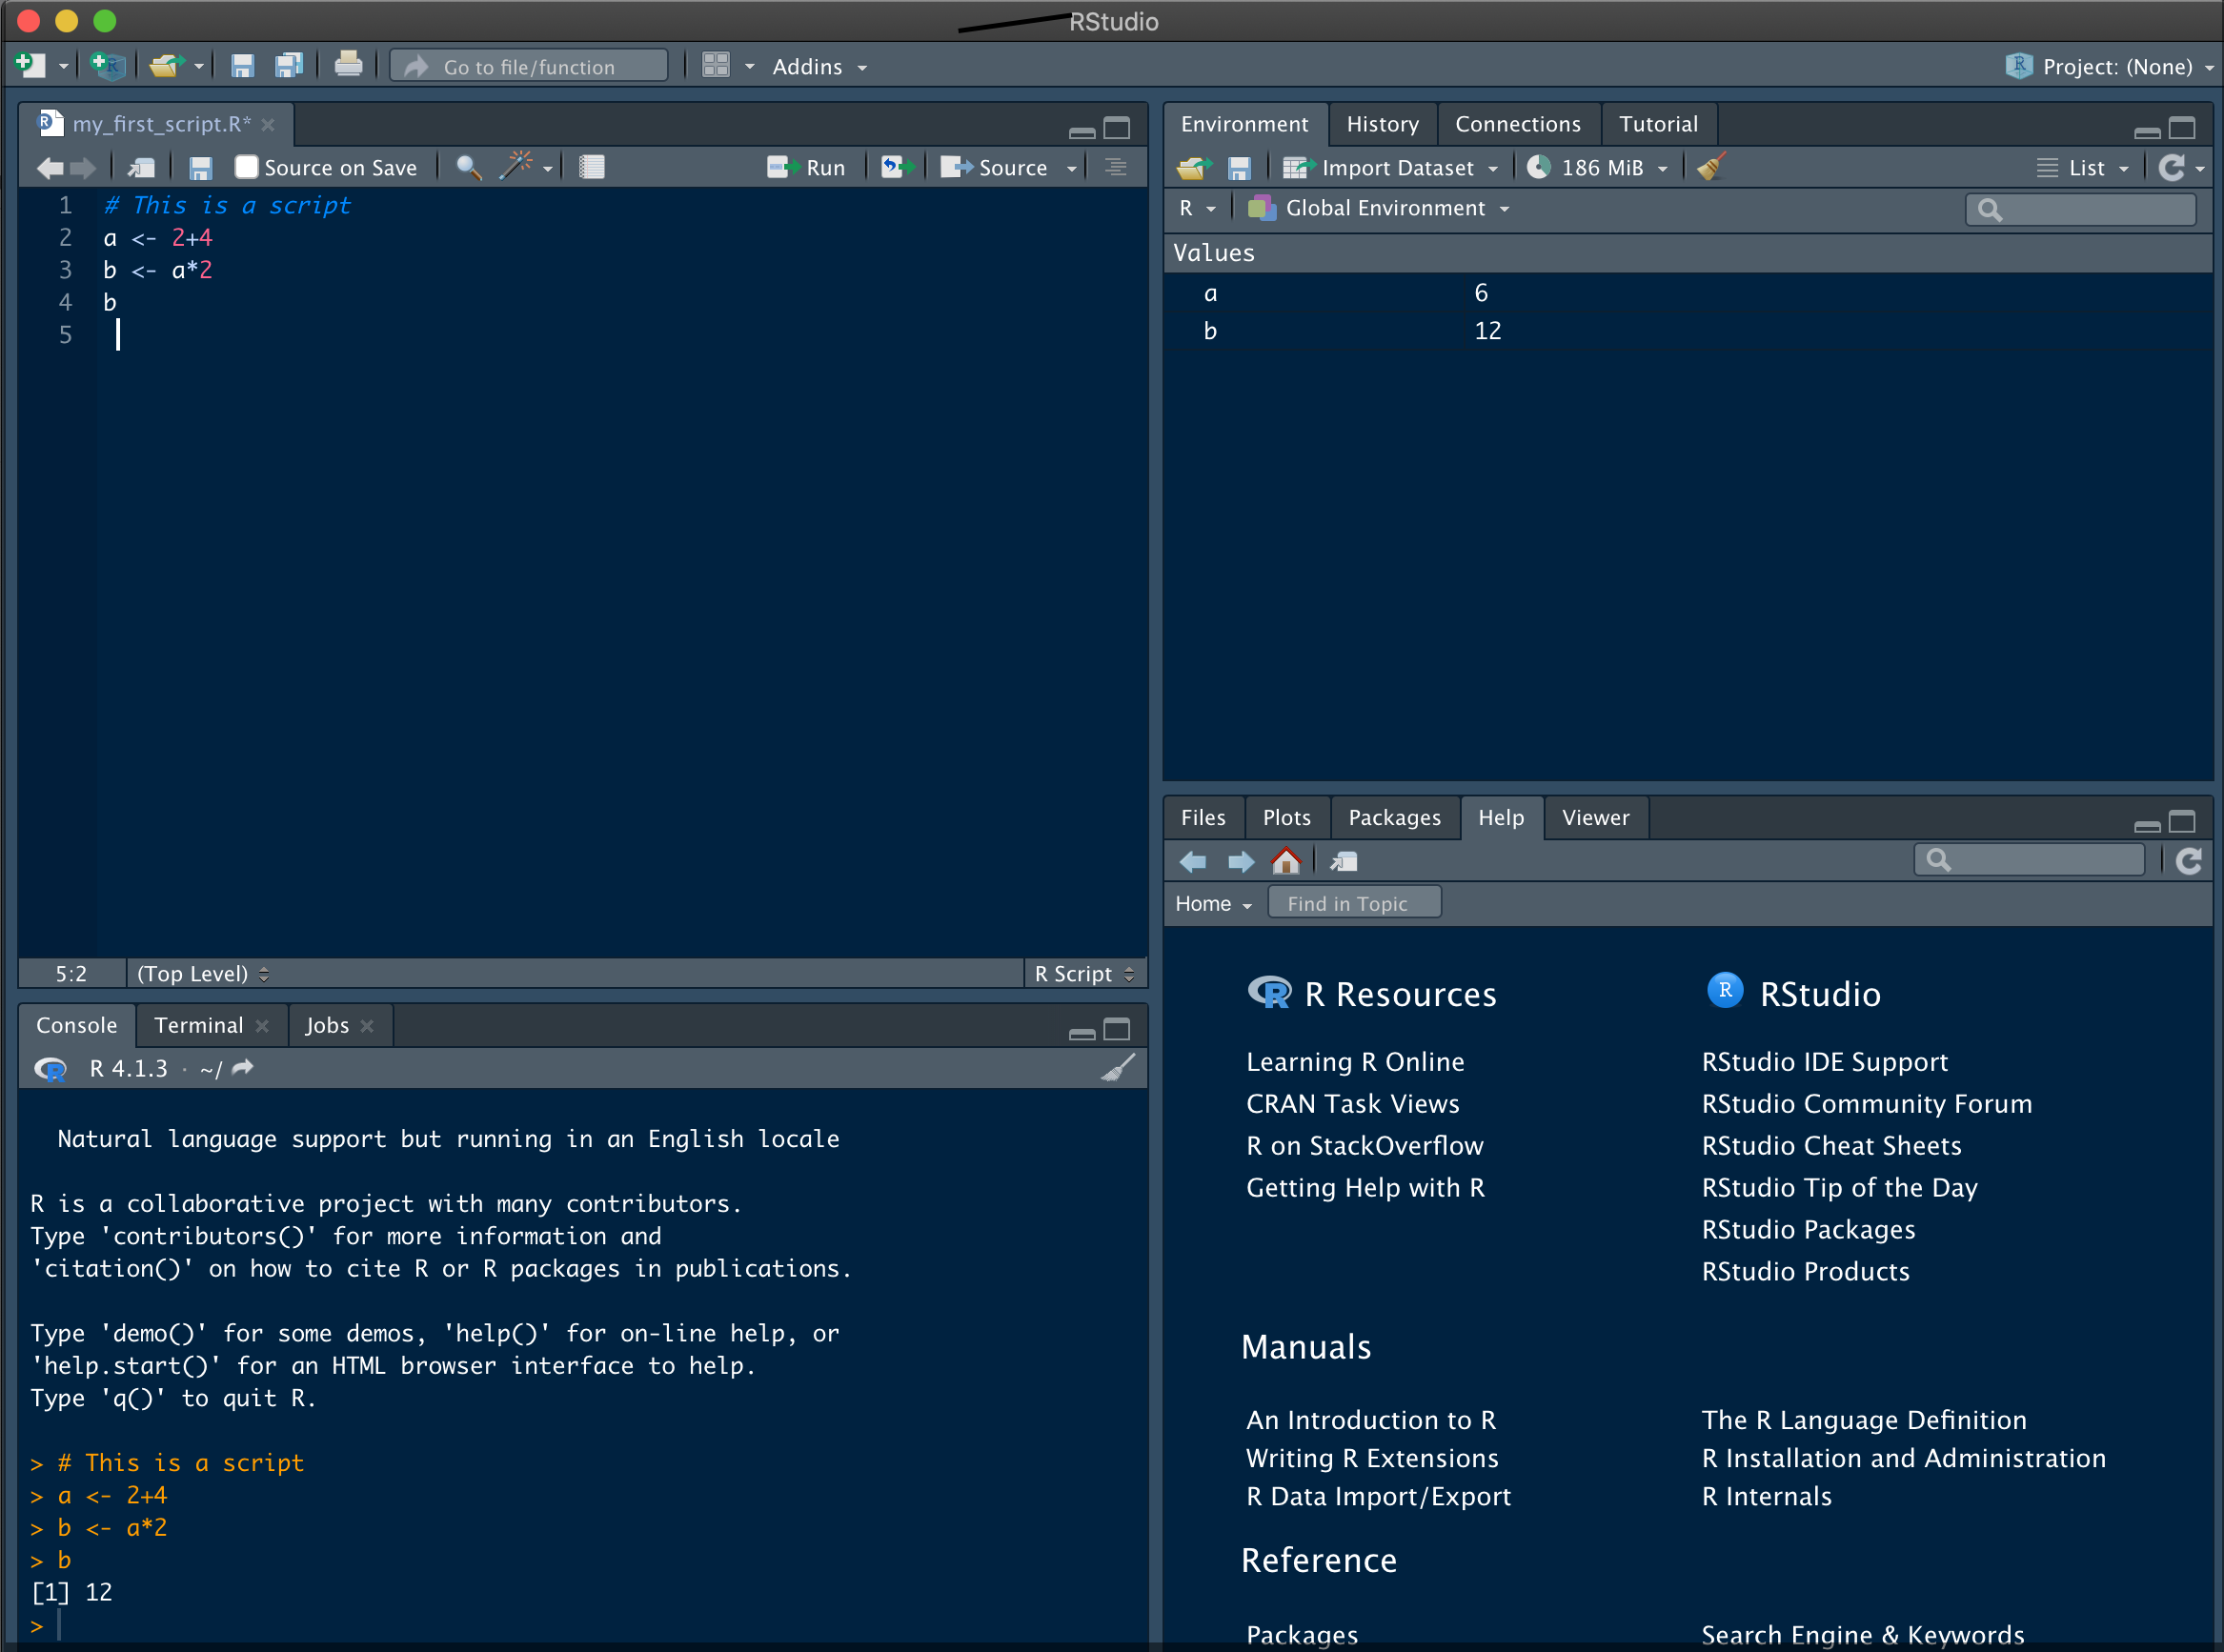
\includegraphics{Rstudio.png}
\caption{Rstudio.png}
\end{figure}

For now, we will focused on the two on the left column. On top, you will have your ``scripting'' window, the place to write and save code. Just below, you have the ``console'' where you can type code directly but also throw lines or full scripts from the window above.

The typical workflow will be to: i) try code in the console, ii) when you're happy with it, save it into your script. This will help you redo whenever and wherever you want your analyses, ie to do some \emph{reproducible} analyses.

At the console, up and down arrows will navigate through your command history. Ctrl+L will erase the console, not the history. You can also access history through the ``History'' tab in RStudio.

On the scripting window, Ctrl+Enter will execute the current line, Maj+Ctrl+B will execute every line from the top of your script to the current line. Use these shortcuts from the very beginning of of your journey into R! Moe of them can be found through Rstudio's menu when you access ``Keyboard shortcuts help''.

\hypertarget{r101}{%
\chapter{R101}\label{r101}}

\hypertarget{hello-world}{%
\section{Hello world}\label{hello-world}}

To follow up the tradition, let's print a message on the console. Open a script, paste the lines below, save it as ``hello.R'' and run it. You can also type it directly into the console.

\begin{Shaded}
\begin{Highlighting}[]
\NormalTok{hello }\OtherTok{\textless{}{-}} \StringTok{"Hello world!"}
\NormalTok{hello}
\end{Highlighting}
\end{Shaded}

\begin{verbatim}
## [1] "Hello world!"
\end{verbatim}

As you can see, R code is pretty natural and easy to read. Usually we read it from right to left (and also from nested brackets to outer brackets).

Here, we have typed a message, explicitly created as a chain of characters because we put it into quotes (\texttt{"})\footnote{You can use simple quotes (\texttt{\textquotesingle{}}) as well. Having two different quotes allow to use one for defining a string, and the other to use as a litteral quote, try: \texttt{print("Hello\ \textquotesingle{}quoted\textquotesingle{}\ world")}}. Then we use the \textbf{assignment operator} \texttt{\textless{}-} whose direction indicates that we assign it into a \textbf{variable} called \texttt{hello}.

When \texttt{hello} is \textbf{called}, it simply prints it message on the console\footnote{R does actually call \texttt{print(hello)} for you}.

\hypertarget{basic-arithmetics}{%
\section{Basic arithmetics}\label{basic-arithmetics}}

You're likely here to manipulate numbers not only strings, so here we go:

\begin{Shaded}
\begin{Highlighting}[]
\NormalTok{x }\OtherTok{\textless{}{-}} \DecValTok{32}\SpecialCharTok{*}\DecValTok{2}
\NormalTok{y }\OtherTok{\textless{}{-}} \FunctionTok{sqrt}\NormalTok{(x)}
\NormalTok{y}
\end{Highlighting}
\end{Shaded}

\begin{verbatim}
## [1] 8
\end{verbatim}

\begin{Shaded}
\begin{Highlighting}[]
\NormalTok{y}\SpecialCharTok{\^{}}\DecValTok{2}
\end{Highlighting}
\end{Shaded}

\begin{verbatim}
## [1] 64
\end{verbatim}

R is a sophisticated calculator that you can use to do basic arithmetics. Here we assigned the result of \texttt{32*2} into a variable called \texttt{x}, then we calculated the square root of \texttt{x} and assigned it to another variable called \texttt{y}. To do so, we used the \texttt{function} \texttt{sqrt()} which is short for square root. When the \texttt{sqrt} function is \emph{passed} with the \textbf{argument} x, the value of the latter is retrived and its square root is returned.

The \texttt{*} and the \texttt{\^{}} are arithmetic \textbf{operators}. You can access all of them by typing \texttt{?Arithmetic} in the console. An operator roughly means ``shortcut'', in other words, a function call to hides its brackets.

\hypertarget{functions-and-help-pages}{%
\section{Functions and help pages}\label{functions-and-help-pages}}

In R, everything that has brackets is a function call\footnote{and more generally everything is a function call in R, even when you do not see brackets (try \texttt{"*"(1,\ 2)}).}.

All functions have a manual page that can be accessed using \texttt{?function\_name}, for example \texttt{?print}. Some general topics are also accessible for example \texttt{?Arithmetic}.

Every time you discover and/or struggle a function, read the manual. Help pages are not exactly poetry: they may appear boring and disturbing at first but there is beauty in their concision and what you're looking for is probably there. Most of them also have examples that you can copy/paste to better understand what they do\footnote{One can also use \texttt{example("function\_name")}}.

\hypertarget{vectors}{%
\section{Vectors}\label{vectors}}

So far, we have only had variables with a single value or \textbf{scalars}. A variable can be a \textbf{vector} and contain more than a single value. To create vectors, we use the function \texttt{c} which names stands for ``concatenate''.

\begin{Shaded}
\begin{Highlighting}[]
\NormalTok{x }\OtherTok{\textless{}{-}} \FunctionTok{c}\NormalTok{(}\DecValTok{1}\NormalTok{, }\DecValTok{2}\NormalTok{, }\DecValTok{3}\NormalTok{, }\DecValTok{4}\NormalTok{, }\DecValTok{5}\NormalTok{, }\DecValTok{6}\NormalTok{, }\DecValTok{7}\NormalTok{)}
\NormalTok{x}\SpecialCharTok{\^{}}\DecValTok{2}
\end{Highlighting}
\end{Shaded}

\begin{verbatim}
## [1]  1  4  9 16 25 36 49
\end{verbatim}

Here we assigned a new value to \texttt{x}, so the previous one (64) is lost. As you can see, when calculating \texttt{x\^{}2}, we calculate the square of all values of \texttt{x}. Not all functions behave this way since some of them return a scalar, by construction:

\begin{Shaded}
\begin{Highlighting}[]
\FunctionTok{length}\NormalTok{(x)}
\end{Highlighting}
\end{Shaded}

\begin{verbatim}
## [1] 7
\end{verbatim}

\begin{Shaded}
\begin{Highlighting}[]
\FunctionTok{sum}\NormalTok{(x)}
\end{Highlighting}
\end{Shaded}

\begin{verbatim}
## [1] 28
\end{verbatim}

\begin{Shaded}
\begin{Highlighting}[]
\FunctionTok{sd}\NormalTok{(x)}
\end{Highlighting}
\end{Shaded}

\begin{verbatim}
## [1] 2.160247
\end{verbatim}

Here we accessed the number of elements in \texttt{x} (with \texttt{length}), its \texttt{sum} and its standard deviation (\texttt{sd}).

Now let say we are interested in calculating the sum of integers not from 1 to 7, but from 1 to 100. As you can imagine, there must be a smarter way than typing \texttt{c(1,\ 2,\ ...,\ 99,\ 100)}. You're right, and that's the job of \texttt{seq}:

\begin{Shaded}
\begin{Highlighting}[]
\FunctionTok{sum}\NormalTok{(}\FunctionTok{seq}\NormalTok{(}\AttributeTok{from=}\DecValTok{1}\NormalTok{, }\AttributeTok{to=}\DecValTok{100}\NormalTok{, }\AttributeTok{by=}\DecValTok{1}\NormalTok{))}
\end{Highlighting}
\end{Shaded}

\begin{verbatim}
## [1] 5050
\end{verbatim}

\hypertarget{the-golden-rule}{%
\section{The golden rule}\label{the-golden-rule}}

Possibly the most important rule in R, and in any programming language is :

\begin{quote}
If something sounds dumb and/or repeatitive there must be a smarter way to do it.
\end{quote}

There are several ways to avoid to do dumb and/or repeative things like having vocabulary (knowing functions to avoid paraphrasing) or the right grammar (ie defining your own functions to avoid copy/pasting entire blocks with minro changes between them). Be sure, that of this will come naturally with time and mistakes. Everything in its time, the first step is to make things work, then the aim will be to doing it in a smarter way.

Back to regular sequences, this is such a repetitive need that we have a shortcut for that, thanks to the operator \texttt{:}.

\begin{Shaded}
\begin{Highlighting}[]
\FunctionTok{sum}\NormalTok{(}\DecValTok{1}\SpecialCharTok{:}\DecValTok{100}\NormalTok{)}
\end{Highlighting}
\end{Shaded}

\begin{verbatim}
## [1] 5050
\end{verbatim}

\hypertarget{function-arguments}{%
\section{Function arguments}\label{function-arguments}}

When using \texttt{seq} as above, you can do more things because there are different flavours of regular sequences. That's the purpose of functions \textbf{arguments}. You can see arguments as functions parameters or options, but we will call them arguments. They are easily recognized because they come into functions brackets. In the code above they were explicitely named so that we know, at first glance, what they do: we \texttt{start} from 1, we go \texttt{to} 100, \texttt{by} an increment of 1.

This does not come out of the blue but from the function \textbf{definition}, that is how the function was written by someone else for you to use it. Have a look to the manual. Past the summary, the second and third section are ``Usage'' and ``Arguments''. Again, everytime you feel that a function could do something that fits your needs, it is probably there and you have to find the information in the manual. For instance if you want, only even numbers, or a sequence of a length 12, it is simply variants of \texttt{seq}:

\begin{Shaded}
\begin{Highlighting}[]
\FunctionTok{seq}\NormalTok{(}\DecValTok{0}\NormalTok{, }\DecValTok{10}\NormalTok{, }\AttributeTok{by=}\DecValTok{2}\NormalTok{)}
\end{Highlighting}
\end{Shaded}

\begin{verbatim}
## [1]  0  2  4  6  8 10
\end{verbatim}

\begin{Shaded}
\begin{Highlighting}[]
\FunctionTok{seq}\NormalTok{(}\DecValTok{0}\NormalTok{, }\DecValTok{10}\NormalTok{, }\AttributeTok{length=}\DecValTok{4}\NormalTok{)}
\end{Highlighting}
\end{Shaded}

\begin{verbatim}
## [1]  0.000000  3.333333  6.666667 10.000000
\end{verbatim}

If you compared the syntax to the Usage section of \texttt{?seq}, you will probably note that above, I omitted the name of the first two arguments (\texttt{from} and \texttt{to}), and also that the third argument was \texttt{by} and then \texttt{length}. I also abbreviated \texttt{length.out} as \texttt{length}, and yet, it works as expected. The rules to know when working with arguments follows:

\begin{itemize}
\tightlist
\item
  You can omit argument names as long as they come in the same order as found in the \texttt{Usage} section.
\item
  You can abbreviate argument names as long as the abbreviation in unequivocal among all defined arguments
\item
  If an argument is not specified, it takes its default value, as mentionned in the Usage section
\item
  You can, yet it is never necessary nor a good idea, change the order of arguments.
\end{itemize}

In other words, these commands are strictly equivalent:

\begin{Shaded}
\begin{Highlighting}[]
\FunctionTok{seq}\NormalTok{(}\AttributeTok{from=}\DecValTok{1}\NormalTok{, }\AttributeTok{to=}\DecValTok{5}\NormalTok{, }\AttributeTok{by=}\FloatTok{1.2}\NormalTok{)}
\end{Highlighting}
\end{Shaded}

\begin{verbatim}
## [1] 1.0 2.2 3.4 4.6
\end{verbatim}

\begin{Shaded}
\begin{Highlighting}[]
\FunctionTok{seq}\NormalTok{(}\AttributeTok{f=}\DecValTok{1}\NormalTok{, }\AttributeTok{t=}\DecValTok{5}\NormalTok{, }\AttributeTok{b=}\FloatTok{1.2}\NormalTok{)}
\end{Highlighting}
\end{Shaded}

\begin{verbatim}
## [1] 1.0 2.2 3.4 4.6
\end{verbatim}

\begin{Shaded}
\begin{Highlighting}[]
\FunctionTok{seq}\NormalTok{(}\DecValTok{1}\NormalTok{, }\DecValTok{5}\NormalTok{, }\FloatTok{1.2}\NormalTok{)}
\end{Highlighting}
\end{Shaded}

\begin{verbatim}
## [1] 1.0 2.2 3.4 4.6
\end{verbatim}

\begin{Shaded}
\begin{Highlighting}[]
\FunctionTok{seq}\NormalTok{(}\AttributeTok{by=}\FloatTok{1.2}\NormalTok{, }\AttributeTok{to=}\DecValTok{5}\NormalTok{)}
\end{Highlighting}
\end{Shaded}

\begin{verbatim}
## [1] 1.0 2.2 3.4 4.6
\end{verbatim}

\hypertarget{other-sequence-generators}{%
\section{Other sequence generators}\label{other-sequence-generators}}

Also have a look to \texttt{rep} that replicated elements of vectors:

\begin{Shaded}
\begin{Highlighting}[]
\FunctionTok{rep}\NormalTok{(}\DecValTok{1}\SpecialCharTok{:}\DecValTok{3}\NormalTok{, }\AttributeTok{each=}\DecValTok{3}\NormalTok{)}
\end{Highlighting}
\end{Shaded}

\begin{verbatim}
## [1] 1 1 1 2 2 2 3 3 3
\end{verbatim}

\begin{Shaded}
\begin{Highlighting}[]
\FunctionTok{rep}\NormalTok{(}\DecValTok{5}\SpecialCharTok{:}\DecValTok{2}\NormalTok{, }\AttributeTok{times=}\DecValTok{2}\NormalTok{)}
\end{Highlighting}
\end{Shaded}

\begin{verbatim}
## [1] 5 4 3 2 5 4 3 2
\end{verbatim}

We will explored them later, but if you are looking for random number generation, they are named \texttt{r+abbreviated\_distribution\_name}:

\begin{Shaded}
\begin{Highlighting}[]
\FunctionTok{set.seed}\NormalTok{(}\DecValTok{123}\NormalTok{)}
\FunctionTok{runif}\NormalTok{(}\DecValTok{5}\NormalTok{, }\DecValTok{0}\NormalTok{, }\DecValTok{1}\NormalTok{)}
\end{Highlighting}
\end{Shaded}

\begin{verbatim}
## [1] 0.2875775 0.7883051 0.4089769 0.8830174 0.9404673
\end{verbatim}

\begin{Shaded}
\begin{Highlighting}[]
\FunctionTok{rnorm}\NormalTok{(}\DecValTok{10}\NormalTok{, }\DecValTok{0}\NormalTok{, }\DecValTok{1}\NormalTok{)}
\end{Highlighting}
\end{Shaded}

\begin{verbatim}
##  [1] -1.6895557  1.2394959 -0.1089660 -0.1172420  0.1830826  1.2805549
##  [7] -1.7272706  1.6901844  0.5038124  2.5283366
\end{verbatim}

\hypertarget{recycling}{%
\section{Recycling}\label{recycling}}

When you do an operation between two vectors, it is usually done element-wise:

\begin{Shaded}
\begin{Highlighting}[]
\NormalTok{x }\OtherTok{\textless{}{-}} \DecValTok{1}\SpecialCharTok{:}\DecValTok{5}
\NormalTok{y }\OtherTok{\textless{}{-}} \DecValTok{10}\SpecialCharTok{:}\DecValTok{6}
\NormalTok{x}
\end{Highlighting}
\end{Shaded}

\begin{verbatim}
## [1] 1 2 3 4 5
\end{verbatim}

\begin{Shaded}
\begin{Highlighting}[]
\NormalTok{y}
\end{Highlighting}
\end{Shaded}

\begin{verbatim}
## [1] 10  9  8  7  6
\end{verbatim}

\begin{Shaded}
\begin{Highlighting}[]
\NormalTok{x}\SpecialCharTok{*}\NormalTok{y}
\end{Highlighting}
\end{Shaded}

\begin{verbatim}
## [1] 10 18 24 28 30
\end{verbatim}

But when the length of vectors is not compatible, R does \textbf{recycle} the shorted vector to match the length of the longer one. Usually, recycling is useful but it may also be troublesome, particularly when it does not come with a warning.

\begin{Shaded}
\begin{Highlighting}[]
\NormalTok{z }\OtherTok{\textless{}{-}} \FunctionTok{c}\NormalTok{(}\DecValTok{0}\NormalTok{, }\DecValTok{1}\NormalTok{)}
\NormalTok{x}
\end{Highlighting}
\end{Shaded}

\begin{verbatim}
## [1] 1 2 3 4 5
\end{verbatim}

\begin{Shaded}
\begin{Highlighting}[]
\NormalTok{z}
\end{Highlighting}
\end{Shaded}

\begin{verbatim}
## [1] 0 1
\end{verbatim}

\begin{Shaded}
\begin{Highlighting}[]
\NormalTok{x}\SpecialCharTok{+}\NormalTok{z }\CommentTok{\# equivalent to c(1, 2, 3, 4, 5) + c(0, 1, 0, 1, 0)}
\end{Highlighting}
\end{Shaded}

\begin{verbatim}
## Warning in x + z: longer object length is not a multiple of shorter object
## length
\end{verbatim}

\begin{verbatim}
## [1] 1 3 3 5 5
\end{verbatim}

\hypertarget{indexing}{%
\section{Indexing}\label{indexing}}

To access a particular element in an object, we will use the square bracket \texttt{object{[}i{]}}, with i being the index of the element to access:

\begin{Shaded}
\begin{Highlighting}[]
\NormalTok{x }\OtherTok{\textless{}{-}} \FunctionTok{c}\NormalTok{(}\DecValTok{3}\NormalTok{, }\DecValTok{1}\NormalTok{, }\DecValTok{5}\NormalTok{, }\DecValTok{4}\NormalTok{)}
\NormalTok{x[}\DecValTok{2}\NormalTok{]}
\end{Highlighting}
\end{Shaded}

\begin{verbatim}
## [1] 1
\end{verbatim}

\begin{Shaded}
\begin{Highlighting}[]
\NormalTok{x[}\DecValTok{3}\NormalTok{]}\SpecialCharTok{/}\DecValTok{4}
\end{Highlighting}
\end{Shaded}

\begin{verbatim}
## [1] 1.25
\end{verbatim}

In R, the first element is 1\footnote{This may sound natural but in most languages it is 0}.

Indexing can be used to access a particular value and/or to change it when combined with the \textbf{assignment operator}

\begin{Shaded}
\begin{Highlighting}[]
\NormalTok{x}
\end{Highlighting}
\end{Shaded}

\begin{verbatim}
## [1] 3 1 5 4
\end{verbatim}

\begin{Shaded}
\begin{Highlighting}[]
\NormalTok{x[}\DecValTok{2}\NormalTok{] }\OtherTok{\textless{}{-}} \FloatTok{1.2}
\NormalTok{x}
\end{Highlighting}
\end{Shaded}

\begin{verbatim}
## [1] 3.0 1.2 5.0 4.0
\end{verbatim}

You can also access more than one element:

\begin{Shaded}
\begin{Highlighting}[]
\NormalTok{x[}\DecValTok{2}\SpecialCharTok{:}\DecValTok{4}\NormalTok{]}
\end{Highlighting}
\end{Shaded}

\begin{verbatim}
## [1] 1.2 5.0 4.0
\end{verbatim}

\begin{Shaded}
\begin{Highlighting}[]
\NormalTok{x[}\FunctionTok{c}\NormalTok{(}\DecValTok{1}\NormalTok{, }\DecValTok{3}\NormalTok{)]}
\end{Highlighting}
\end{Shaded}

\begin{verbatim}
## [1] 3 5
\end{verbatim}

And change more than a single value at a time. Recycling applies here

\begin{Shaded}
\begin{Highlighting}[]
\NormalTok{x}
\end{Highlighting}
\end{Shaded}

\begin{verbatim}
## [1] 3.0 1.2 5.0 4.0
\end{verbatim}

\begin{Shaded}
\begin{Highlighting}[]
\NormalTok{x[}\DecValTok{2}\SpecialCharTok{:}\DecValTok{4}\NormalTok{] }\OtherTok{\textless{}{-}} \FunctionTok{c}\NormalTok{(}\FloatTok{0.2}\NormalTok{, }\FloatTok{0.4}\NormalTok{, }\FloatTok{0.5}\NormalTok{)}
\NormalTok{x}
\end{Highlighting}
\end{Shaded}

\begin{verbatim}
## [1] 3.0 0.2 0.4 0.5
\end{verbatim}

\begin{Shaded}
\begin{Highlighting}[]
\NormalTok{x[}\DecValTok{2}\SpecialCharTok{:}\DecValTok{4}\NormalTok{] }\OtherTok{\textless{}{-}} \DecValTok{99}
\NormalTok{x}
\end{Highlighting}
\end{Shaded}

\begin{verbatim}
## [1]  3 99 99 99
\end{verbatim}

So far we have seed \textbf{positive indexing} but sometimes it is also useful to state which elements you do NOT want:

\begin{Shaded}
\begin{Highlighting}[]
\NormalTok{x }\OtherTok{\textless{}{-}} \DecValTok{3}\SpecialCharTok{:}\DecValTok{7}
\NormalTok{x}
\end{Highlighting}
\end{Shaded}

\begin{verbatim}
## [1] 3 4 5 6 7
\end{verbatim}

\begin{Shaded}
\begin{Highlighting}[]
\NormalTok{x[}\SpecialCharTok{{-}}\DecValTok{1}\NormalTok{] }\CommentTok{\# all but the first}
\end{Highlighting}
\end{Shaded}

\begin{verbatim}
## [1] 4 5 6 7
\end{verbatim}

\begin{Shaded}
\begin{Highlighting}[]
\NormalTok{x[}\SpecialCharTok{{-}}\FunctionTok{length}\NormalTok{(x)] }\CommentTok{\# all but the last}
\end{Highlighting}
\end{Shaded}

\begin{verbatim}
## [1] 3 4 5 6
\end{verbatim}

\begin{Shaded}
\begin{Highlighting}[]
\NormalTok{x[}\SpecialCharTok{{-}}\FunctionTok{c}\NormalTok{(}\DecValTok{1}\NormalTok{, }\FunctionTok{length}\NormalTok{(x))] }\CommentTok{\# trim both ends}
\end{Highlighting}
\end{Shaded}

\begin{verbatim}
## [1] 4 5 6
\end{verbatim}

You can also use variables:

\begin{Shaded}
\begin{Highlighting}[]
\NormalTok{indices }\OtherTok{\textless{}{-}} \FunctionTok{c}\NormalTok{(}\DecValTok{1}\NormalTok{, }\DecValTok{4}\NormalTok{)}
\NormalTok{x }\OtherTok{\textless{}{-}} \SpecialCharTok{{-}}\DecValTok{2}\SpecialCharTok{:}\DecValTok{3}
\NormalTok{x}
\end{Highlighting}
\end{Shaded}

\begin{verbatim}
## [1] -2 -1  0  1  2  3
\end{verbatim}

\begin{Shaded}
\begin{Highlighting}[]
\NormalTok{x[indices]}
\end{Highlighting}
\end{Shaded}

\begin{verbatim}
## [1] -2  1
\end{verbatim}

\hypertarget{tests-and-logicals}{%
\section{Tests and logicals}\label{tests-and-logicals}}

You can do logical tests in R. They return a vector of type ``logical''.

\begin{Shaded}
\begin{Highlighting}[]
\NormalTok{x }\OtherTok{\textless{}{-}} \DecValTok{1}\SpecialCharTok{:}\DecValTok{5}
\NormalTok{x }\SpecialCharTok{\textgreater{}} \DecValTok{3}
\end{Highlighting}
\end{Shaded}

\begin{verbatim}
## [1] FALSE FALSE FALSE  TRUE  TRUE
\end{verbatim}

You can directly pass this vector of type \texttt{logical} as an indexing variable or turn them into \texttt{numeric} indices:

\begin{Shaded}
\begin{Highlighting}[]
\NormalTok{x[x }\SpecialCharTok{\textgreater{}} \DecValTok{3}\NormalTok{]}
\end{Highlighting}
\end{Shaded}

\begin{verbatim}
## [1] 4 5
\end{verbatim}

\begin{Shaded}
\begin{Highlighting}[]
\NormalTok{above\_three }\OtherTok{\textless{}{-}} \FunctionTok{which}\NormalTok{(x}\SpecialCharTok{\textgreater{}}\DecValTok{3}\NormalTok{)}
\NormalTok{x[above\_three]}
\end{Highlighting}
\end{Shaded}

\begin{verbatim}
## [1] 4 5
\end{verbatim}

To get the full list of relational operators, type \texttt{?Comparison}. You can also do set operations, see \texttt{?sets}; \texttt{\%in\%} operator is often used

\begin{Shaded}
\begin{Highlighting}[]
\NormalTok{x}
\end{Highlighting}
\end{Shaded}

\begin{verbatim}
## [1] 1 2 3 4 5
\end{verbatim}

\begin{Shaded}
\begin{Highlighting}[]
\NormalTok{x}\SpecialCharTok{==}\DecValTok{4}
\end{Highlighting}
\end{Shaded}

\begin{verbatim}
## [1] FALSE FALSE FALSE  TRUE FALSE
\end{verbatim}

\begin{Shaded}
\begin{Highlighting}[]
\NormalTok{x}\SpecialCharTok{\textless{}=}\DecValTok{3}
\end{Highlighting}
\end{Shaded}

\begin{verbatim}
## [1]  TRUE  TRUE  TRUE FALSE FALSE
\end{verbatim}

\begin{Shaded}
\begin{Highlighting}[]
\NormalTok{x}\SpecialCharTok{!=}\DecValTok{2}
\end{Highlighting}
\end{Shaded}

\begin{verbatim}
## [1]  TRUE FALSE  TRUE  TRUE  TRUE
\end{verbatim}

\begin{Shaded}
\begin{Highlighting}[]
\NormalTok{x }\SpecialCharTok{\%in\%} \FunctionTok{c}\NormalTok{(}\DecValTok{2}\NormalTok{, }\DecValTok{4}\NormalTok{)}
\end{Highlighting}
\end{Shaded}

\begin{verbatim}
## [1] FALSE  TRUE FALSE  TRUE FALSE
\end{verbatim}

\hypertarget{na}{%
\section{NA}\label{na}}

\begin{Shaded}
\begin{Highlighting}[]
\NormalTok{x[}\FunctionTok{seq}\NormalTok{(}\DecValTok{1}\NormalTok{, }\DecValTok{5}\NormalTok{, }\AttributeTok{by=}\DecValTok{2}\NormalTok{)]}
\end{Highlighting}
\end{Shaded}

\begin{verbatim}
## [1] 1 3 5
\end{verbatim}

On the last command, we tried to access all elements from 1 to 5 with an increment of 2 (ie \texttt{\{1,\ 3,\ 5\}}). The \texttt{x} only has 4 elements, so the 5\^{}th does not exist. R returns \texttt{NA} which stands for \textbf{Non available}. NAs are very common when doing data analyses and some functions may not work as expected as long as there is a single NA in the object you're doing calculations with:

\begin{Shaded}
\begin{Highlighting}[]
\NormalTok{x }\OtherTok{\textless{}{-}} \FunctionTok{c}\NormalTok{(}\DecValTok{1}\NormalTok{, }\DecValTok{5}\NormalTok{, }\ConstantTok{NA}\NormalTok{, }\DecValTok{6}\NormalTok{)}
\FunctionTok{mean}\NormalTok{(x)}
\end{Highlighting}
\end{Shaded}

\begin{verbatim}
## [1] NA
\end{verbatim}

\texttt{NA} is returned here for a good reason: the missing value could be 4 or 3 billions! If you want to ignore NAs, you must explicitely mention it to R. Some functions have a \texttt{na.rm} (remove NAs) arguments, otherwise there is the \texttt{na.omit} function:

\begin{Shaded}
\begin{Highlighting}[]
\FunctionTok{mean}\NormalTok{(x, }\AttributeTok{na.rm=}\ConstantTok{TRUE}\NormalTok{)}
\end{Highlighting}
\end{Shaded}

\begin{verbatim}
## [1] 4
\end{verbatim}

\begin{Shaded}
\begin{Highlighting}[]
\FunctionTok{mean}\NormalTok{(}\FunctionTok{na.omit}\NormalTok{(x))}
\end{Highlighting}
\end{Shaded}

\begin{verbatim}
## [1] 4
\end{verbatim}

\hypertarget{other-structures}{%
\section{Other structures}\label{other-structures}}

Besides scalars and vectors, R can handle objects with more dimensions such as \textbf{matrices} which are 2-dimensionnal \textbf{arrays}, \textbf{lists} and \textbf{data.frame} that are rectangular lists.

\hypertarget{matrices}{%
\subsection{Matrices}\label{matrices}}

Let's begin with matrices:

\begin{Shaded}
\begin{Highlighting}[]
\NormalTok{mat }\OtherTok{\textless{}{-}} \FunctionTok{matrix}\NormalTok{(}\DecValTok{1}\SpecialCharTok{:}\DecValTok{9}\NormalTok{, }\AttributeTok{nrow=}\DecValTok{3}\NormalTok{, }\AttributeTok{ncol=}\DecValTok{3}\NormalTok{)}
\NormalTok{mat}
\end{Highlighting}
\end{Shaded}

\begin{verbatim}
##      [,1] [,2] [,3]
## [1,]    1    4    7
## [2,]    2    5    8
## [3,]    3    6    9
\end{verbatim}

Matrices are rectangular objects that contain number on which we can do many thing, including arithmetic operations:

\begin{Shaded}
\begin{Highlighting}[]
\FunctionTok{sum}\NormalTok{(mat)}
\end{Highlighting}
\end{Shaded}

\begin{verbatim}
## [1] 45
\end{verbatim}

\begin{Shaded}
\begin{Highlighting}[]
\NormalTok{mat}\SpecialCharTok{/}\DecValTok{2}
\end{Highlighting}
\end{Shaded}

\begin{verbatim}
##      [,1] [,2] [,3]
## [1,]  0.5  2.0  3.5
## [2,]  1.0  2.5  4.0
## [3,]  1.5  3.0  4.5
\end{verbatim}

\begin{Shaded}
\begin{Highlighting}[]
\FunctionTok{colSums}\NormalTok{(mat)}
\end{Highlighting}
\end{Shaded}

\begin{verbatim}
## [1]  6 15 24
\end{verbatim}

They can be indexed using the syntax: \texttt{object{[}i,\ j{]}}. We have one more indexing argument, since we now have two dimensions. The first being the row index, the second being the column index by convention. If you omit one, this means ``take all of them''. Otherwise, all other indexing rules applies.

\begin{Shaded}
\begin{Highlighting}[]
\NormalTok{mat[}\DecValTok{1}\NormalTok{, }\DecValTok{2}\NormalTok{] }\CommentTok{\# first row, second column}
\end{Highlighting}
\end{Shaded}

\begin{verbatim}
## [1] 4
\end{verbatim}

\begin{Shaded}
\begin{Highlighting}[]
\NormalTok{mat[}\DecValTok{2}\NormalTok{, ] }\CommentTok{\# second row}
\end{Highlighting}
\end{Shaded}

\begin{verbatim}
## [1] 2 5 8
\end{verbatim}

\begin{Shaded}
\begin{Highlighting}[]
\NormalTok{mat[}\SpecialCharTok{{-}}\DecValTok{2}\NormalTok{, }\FunctionTok{c}\NormalTok{(}\DecValTok{1}\NormalTok{, }\DecValTok{3}\NormalTok{)] }\CommentTok{\# all rows but the second, first and third columns}
\end{Highlighting}
\end{Shaded}

\begin{verbatim}
##      [,1] [,2]
## [1,]    1    7
## [2,]    3    9
\end{verbatim}

Among useful functions when working with matrices, we have:

\begin{Shaded}
\begin{Highlighting}[]
\FunctionTok{dim}\NormalTok{(mat) }
\end{Highlighting}
\end{Shaded}

\begin{verbatim}
## [1] 3 3
\end{verbatim}

\begin{Shaded}
\begin{Highlighting}[]
\FunctionTok{nrow}\NormalTok{(mat)}
\end{Highlighting}
\end{Shaded}

\begin{verbatim}
## [1] 3
\end{verbatim}

\begin{Shaded}
\begin{Highlighting}[]
\FunctionTok{ncol}\NormalTok{(mat)}
\end{Highlighting}
\end{Shaded}

\begin{verbatim}
## [1] 3
\end{verbatim}

\begin{Shaded}
\begin{Highlighting}[]
\FunctionTok{colnames}\NormalTok{(mat) }\CommentTok{\# not defined so far}
\end{Highlighting}
\end{Shaded}

\begin{verbatim}
## NULL
\end{verbatim}

\begin{Shaded}
\begin{Highlighting}[]
\FunctionTok{colnames}\NormalTok{(mat) }\OtherTok{\textless{}{-}} \FunctionTok{c}\NormalTok{(}\StringTok{"a"}\NormalTok{, }\StringTok{"b"}\NormalTok{, }\StringTok{"c"}\NormalTok{) }\CommentTok{\# let\textquotesingle{}s name columns}
\FunctionTok{colnames}\NormalTok{(mat) }\CommentTok{\# now defined}
\end{Highlighting}
\end{Shaded}

\begin{verbatim}
## [1] "a" "b" "c"
\end{verbatim}

\hypertarget{lists}{%
\subsection{Lists}\label{lists}}

Lists are vectors than can contain objects of different type. They can be named or not:

\begin{Shaded}
\begin{Highlighting}[]
\NormalTok{x }\OtherTok{\textless{}{-}} \FunctionTok{list}\NormalTok{(}\AttributeTok{a=}\DecValTok{1}\NormalTok{, }\AttributeTok{b=}\StringTok{"hello"}\NormalTok{, }\AttributeTok{c=}\NormalTok{mat)}
\NormalTok{x}
\end{Highlighting}
\end{Shaded}

\begin{verbatim}
## $a
## [1] 1
## 
## $b
## [1] "hello"
## 
## $c
##      a b c
## [1,] 1 4 7
## [2,] 2 5 8
## [3,] 3 6 9
\end{verbatim}

They can be indexed with three different syntaxes: \texttt{{[}}, \texttt{{[}{[}} or \texttt{\$}. \texttt{\$} will only work for a \textbf{single} and \textbf{named} element:

\begin{Shaded}
\begin{Highlighting}[]
\NormalTok{x}\SpecialCharTok{$}\NormalTok{mat}
\end{Highlighting}
\end{Shaded}

\begin{verbatim}
## NULL
\end{verbatim}

This is mostly useful when working with \texttt{data.frame}s that are a particular flavor of lists, to retrieve a single column. We will be back at it later.

Single and double square brackets are quite confusing at first glance, but they allow to retrieve either the element and retain its list nature (\texttt{{[}}), or the element and dropping its list nature (\texttt{{[}{[}}):

\begin{Shaded}
\begin{Highlighting}[]
\NormalTok{x[}\DecValTok{1}\NormalTok{]}
\end{Highlighting}
\end{Shaded}

\begin{verbatim}
## $a
## [1] 1
\end{verbatim}

\begin{Shaded}
\begin{Highlighting}[]
\FunctionTok{class}\NormalTok{(x[}\DecValTok{1}\NormalTok{])}
\end{Highlighting}
\end{Shaded}

\begin{verbatim}
## [1] "list"
\end{verbatim}

\begin{Shaded}
\begin{Highlighting}[]
\CommentTok{\# x[1] + 3 This won\textquotesingle{}t work as we still have a list}

\NormalTok{x[[}\DecValTok{1}\NormalTok{]]}
\end{Highlighting}
\end{Shaded}

\begin{verbatim}
## [1] 1
\end{verbatim}

\begin{Shaded}
\begin{Highlighting}[]
\FunctionTok{class}\NormalTok{(x[[}\DecValTok{1}\NormalTok{]])}
\end{Highlighting}
\end{Shaded}

\begin{verbatim}
## [1] "numeric"
\end{verbatim}

\begin{Shaded}
\begin{Highlighting}[]
\NormalTok{x[[}\DecValTok{1}\NormalTok{]]}\SpecialCharTok{+}\DecValTok{3}
\end{Highlighting}
\end{Shaded}

\begin{verbatim}
## [1] 4
\end{verbatim}

\hypertarget{data.frames}{%
\subsection{data.frames}\label{data.frames}}

Data frames are rectangular lists. They are the natural structure in data analysis because they correspond to a spreadheet.

Consequently and practically, they also are the central object in modern R, at the very core of the tidyverse grammar.

\hypertarget{footnotes}{%
\section{Footnotes}\label{footnotes}}

  \bibliography{book.bib,packages.bib}

\end{document}
